\documentclass[11pt]{article}

% --- Packages ---
\usepackage{amsmath, amssymb, amsthm}
\usepackage{graphicx}
\usepackage{bm}
\usepackage{tikz}
\usepackage{hyperref}
\usepackage{enumitem}

\title{Differance-Integrated Fixed-Point Diffusion: \\
A Structural-Dynamical Hybrid Framework and Its Application to Cross-Species Body-Language Interfaces}

\author{Masaomi Chiba}

\date{\today}

\begin{document}

\maketitle

\begin{abstract}
We propose \emph{Differance-Integrated Fixed-Point Diffusion} (DIFD), a general-purpose 
framework combining isotropic diffusion processes with a non-equilibrium structural operator 
derived from the Derridean notion of \emph{diff\'erance}. The DIFD update rule integrates 
a symmetric noise term with an asymmetric, history-sensitive structural gradient.
This hybrid mechanism allows an agent or model to search not only within a 
likelihood-driven manifold but also across structural variations that are typically 
ignored by purely statistical samplers.

A formal definition of orthogonality between diffusion noise and structural gradient is 
provided, along with empirical validation protocols. As a concrete application, we 
demonstrate how DIFD enables the construction of a ``cross-species body-language 
interface''---a tool that infers and synthesizes body-language cues enabling humans to 
communicate more effectively with domestic animals, focusing on cats as a primary example.
\end{abstract}

\section{Introduction}

Diffusion models have become a core generative paradigm, typically exploring a data 
manifold through noise-perturbed score matching. However, these models remain restricted 
by the statistical structure of the data distribution. They lack a mechanism to traverse 
\emph{structural} alternatives---variations in meaning, relationality, or tacit behaviour 
that are not simply captured by likelihood gradients.

To address this, we introduce \emph{Differance-Integrated Fixed-Point Diffusion} (DIFD), 
which augments diffusion dynamics with a structural correction term inspired by Derrida's 
\emph{diff\'erance}: the notion that meaning arises from both difference and deferred 
relation across representations. The structural component is formalized as a non-symmetric 
``difference operator'' acting as a gradient of a cost functional $C$ defined over 
relational structures rather than mere pointwise data.

One surprising consequence is that the hybrid sampler, when properly tuned, can be used 
to synthesize relational cues for embodied systems. This enables applications such as 
cross-species body-language mediation for animal behaviour support.

\section{Differance-Integrated Fixed-Point Diffusion}

\subsection{Update rule}

Let $z_t \in \mathcal{Z}$ be the latent state at time $t$. DIFD applies the update
\begin{equation}
z_{t+1} = z_t + \epsilon_t - \lambda_t \nabla_z C(z_t),
\end{equation}
where $\epsilon_t \sim \mathcal{N}(0, \sigma_t^2 I)$ is isotropic diffusion noise
and $C$ is a structural cost functional.

The cost $C$ can encode:
\begin{itemize}[itemsep=2pt]
    \item relational asymmetries,
    \item deferred dependencies (temporal or multi-scale),
    \item behavioural counterfactuals,
    \item morphological constraints.
\end{itemize}

Thus $\nabla C$ introduces structural bias rather than statistical bias.

\subsection{Interpretation as hybrid search}

Diffusion drives isotropic local exploration; the DIFW operator drives directed 
structural movement. When orthogonality (defined below) approximately holds, the components 
decouple, enabling efficient structural traversal without corrupting stability.

\section{Formal Orthogonality}

\subsection{Definitions}

Let $g_t := \nabla_z C(z_t)$.

\paragraph{Second-moment orthogonality.}
\begin{equation}
\mathrm{Cov}(\epsilon_t, g_t) = \mathbb{E}[\epsilon_t g_t^\top] = 0.
\end{equation}

\paragraph{Information-theoretic orthogonality.}
\[
I(\epsilon_t; g_t) \approx 0.
\]

\subsection{Why orthogonality matters}

Consider:
\[
\mathbb{E}\|z_{t+1}-z_t\|^2
= \mathbb{E}\|\epsilon_t\|^2 + \lambda_t^2 \mathbb{E}\|g_t\|^2
- 2\lambda_t \operatorname{Tr}(\mathbb{E}[\epsilon_t g_t^\top]).
\]

Under orthogonality the cross-term vanishes.

\subsection{Geometric sufficient condition}

Let $\Sigma_t = \mathrm{Cov}(\epsilon_t)$. If $g_t$ lies largely in the subspace 
corresponding to small eigenvalues of $\Sigma_t$, the covariance vanishes.  
With isotropic noise this reduces to the requirement that $g_t$ has zero expected 
correlation with $\epsilon_t$.

\subsection{Empirical validation}

We recommend the following tests:
\begin{enumerate}[itemsep=3pt]
    \item empirical cross-covariance test,
    \item directional correlation profile against principal axes of $\epsilon_t$,
    \item mutual information estimation (e.g.\ k-NN estimator),
    \item intervention: enforce alignment between $g_t$ and noise directions and measure degradation.
\end{enumerate}

\subsection{Illustration}

\begin{figure}[h]
\centering
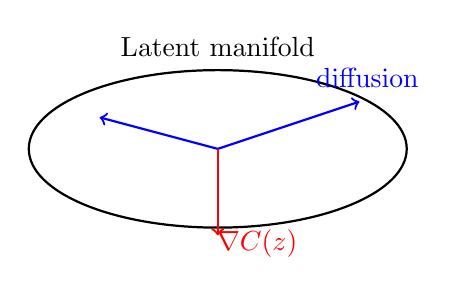
\begin{tikzpicture}[scale=1.0]
  \draw[thick] (0,0) ellipse (2.4cm and 1.0cm);
  \node at (0,1.3) {Latent manifold};

  \draw[->, thick, blue] (0,0) -- (1.8,0.6);
  \draw[->, thick, blue] (0,0) -- (-1.5,0.4);
  \node[blue] at (1.9,0.9) {diffusion};

  \draw[->, thick, red] (0,0) -- (0,-1.1);
  \node[red] at (0.5,-1.2) {$\nabla C(z)$};
\end{tikzpicture}
\caption{Diffusion directions and DIFW gradient approximately orthogonal.}
\end{figure}

\section{Application: Cross-Species Body-Language Interface for Cats}

The core insight is that DIFD separates:
\begin{itemize}
    \item \emph{likelihood-driven} motion patterns learned from data,
    \item \emph{structural body-language operators} capturing deferred relational states.
\end{itemize}

This makes it suitable for a behavioural mediator bridging species with distinct
semiotic systems.

\subsection{Modelling feline body-language structures}

Cat body language involves:
\begin{itemize}[itemsep=3pt]
    \item tail orientation,
    \item ear rotation,
    \item paw tension,
    \item dorsal curvature,
    \item micro-movements of whiskers.
\end{itemize}

These variables are *not* independent. For example:
\[
\text{ear angle} \to \text{tail motion} \to \text{pupil dilation}
\]
forms a deferred dependency chain. Let $C(z)$ encode the mismatch between 
these relational constraints and candidate generative outputs.

\subsection{Body-language synthesis}

Given a human cue $h$, we sample a feline-compatible pose $z$ from:
\[
z = \mathrm{DIFD}(h).
\]

Examples:
\begin{itemize}[itemsep=2pt]
    \item generating a non-threatening crouch posture,
    \item indicating invitation-to-approach with slow-tail-swivel,
    \item conveying playfulness without predatory misinterpretation.
\end{itemize}

\subsection{Behavioural mediation tool}

The final tool consists of:
\begin{enumerate}[itemsep=3pt]
    \item a vision module capturing cat posture,
    \item a latent translator mapping to relational state,
    \item a DIFD sampler generating compatible human-body cues,
    \item a feedback loop for continuous adjustment.
\end{enumerate}

The structural operator prevents the system from producing statistically plausible
poses that nevertheless violate the tacit relational grammar of feline behaviour.

\section{Conclusion}

We introduced DIFD, a framework integrating symmetric diffusion with 
asymmetric relational structure. A formal orthogonality assumption is provided 
with validation protocols. Finally, we demonstrated how DIFD naturally supports 
generative relational mediation tasks, including a cross-species 
body-language interface enabling safer, more intuitive interaction with cats.

\bibliographystyle{plain}
\begin{thebibliography}{9}

\bibitem{score}
Song, Yang, et al.
\emph{Score-Based Generative Modeling}. (2021)

\bibitem{diff}
Sohl-Dickstein, Jascha, et al.
\emph{Deep Unsupervised Learning using Nonequilibrium Thermodynamics}. (2015)

\end{thebibliography}

\end{document}

